
\subsection{Reveiwer Comments - \me{1}}

In this paper, the authors proposed a traffic aware resource allocation scheme for multi-cell MIMO-OFDM systems, where the precoders at all BSs are chosen to minimize the total user queue deviations. The problem is nonconvex and the authors proposed two centralized algorithms based on the successive approximation (SCA) technique to find a stationary point. Moreover, several distributed algorithms are also proposed using primal decomposition, alternating directions method of multipliers (ADMM), and decomposition via KKT conditions, respectively.

Most sections of this paper are well written. The results and algorithms also seem valid. However, the motivation of minimizing the total user queue deviations is not well justified. The convergence results of some algorithms are not clearly presented. The presentation of the distributed solutions needs significant improvement. Analysis and comparison of the signaling overhead and computational complexity between the centralized and distributed algorithms are also necessary to justify the advantages of distributed algorithms.

\resp We thank the reviewer for reading the paper and providing the comments. Please consider the responses in line with the comments.

\subsection*{Detailed Comments}  
\cmnt{1} In Section II.B, please provides more justifications for the problem formulation in (6). For example, the Queue weighted sum rate maximization (Q-WSRM) is throughput optimal, i.e., if there exists a scheme which can make all queues stable, then the Q-WSRM can also do this. How about the proposed formulation in (6)? Is it also throughput optimal? 

\resp We fully agree with the reviewer comment. The Q-WSRM scheme is throughput optimal when the queues associated with the users are significantly large in comparison with the transmission rate (service rate). In order to restrict the over allocation of the available resources to a specific user beyond the total number of queued packets, we have included the additional rate constraint in the Q-WSRME algorithm. It would be ideal to compare with the Q-WSRME algorithm which performs similar to the Q-WSRM when the queued packets are large enough to be emptied by the current transmissions. Fig. \ref{fig-review} compares the centralized algorithms using average number of backlogged packets after \me{100} slots of transmission for different arrival rate. Note that the average arrival rate of all the users are same but the instantaneous arrivals are based on the Poisson distribution. It can be seen from Fig. \ref{fig-review} that the JSFRA scheme with \me{q=2} performs similar to the Q-WSRME scheme for higher arrival rates, which explains the dropping of the squared rate term in the Q-WSRM formulation. When the average arrival rate is smaller, the JSFRA scheme with \me{q=2} performs noticeably better than the Q-WSRME scheme as can be seen from the average number of backlogged packets. In all packet arrival scenarios, JSFRA scheme with \me{q=1} reduces the average number of backlogged packets over the given slots is lesser than the Q-WSRME scheme.
\begin{figure}
\centering
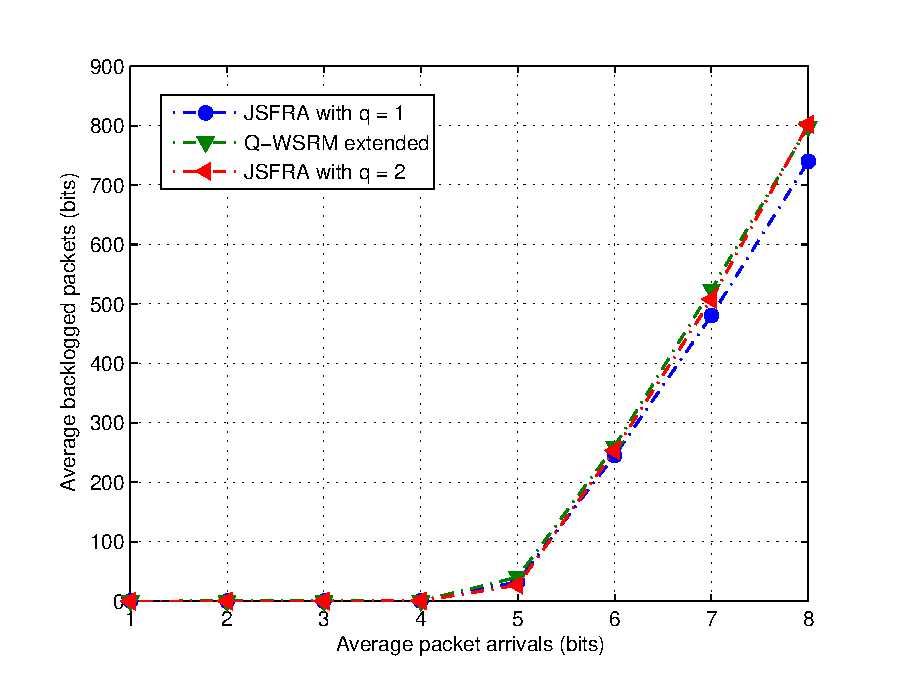
\includegraphics[width=\columnwidth]{Review/reviewer.eps}
\label{fig-review}
\caption{System \me{\lbrace N,N_B,K,N_R \rbrace = \lbrace 4,2,12,1 \rbrace}}
\end{figure}

\cmnt{2} Do the proposed solutions based on (6) achieve better average delay performance than the existing solutions? By the way, in the simulations, you should also add a figure comparing the average delay performance, instead of just comparing the performance metric defined by (6). This will better justify the advantage of the proposed solutions.

\resp We agree with the reviewer comment on the better average delay performance of Q-WSRM(E) approach over JSFRA scheme with \me{q=1} formulation. Note that the average delay can be reduced by including a convex minimum rate constraint in the JSFRA formulation to provide a guaranteed rate to all users or for certain users in the system. More over, the priority can also be incorporated easily in the formulation by the scaling factor \me{a_k} used in the formulation. As mentioned in Section \ref{sec-3.2}, the delay can also be addressed by using \me{q=2} or \me{q=\infty} norm objective in the JSFRA formulation.

\cmnt{3} In Section III.B, the convergence conditions under Algorithm 1 are not clear. First, you should be more specific about what is the SCA subproblem. Do you mean problem (19)? Second, does the uniqueness of the transmit and receive beamformers mean that the solution of the original problem in (16) is unique, or the solutions of the subproblems in (19) and (20) are unique, respectively?

\resp We understand the reviewer concerns. We have modified the convergence section to include additional information to provide more clarity. \review{Update converge proof}

\cmnt{4} It is better to clearly summarize the convergence conditions and results (i.e., does it converge to a stationary point or the optimal solution) for all algorithms in a theorem/proposition.

\resp We agree with the reviewers view. We have updated the convergence proof to include the discussions on the stationary point and the optimal point.

\cmnt{5} At the end of Section III, you mentioned that the proposed reduced complexity resource allocation scheme is sensitive to the order in which the subchannels are selected for the optimization problem. Please provide a discussion how to choose this order.

\resp We thank the reviewer for the raising the concern on the selection order. We have elaborated the discussion on the sub-channel wise selection scheme. \review{discuss on selection}

\cmnt{6} In the distributed algorithms, it is not clear what exact information is exchanged between the BSs or between the BSs and users. Moreover, the signaling overhead should be analyzed and compared with the centralized solution. The proposed distributed algorithms require exchanging over-the-air signaling or backhaul signaling for many times within each channel coherent time (e.g., from Fig. 2, the distributed algorithm requires 20-30 iterations to converge even when there are only 3 subchannels). I don’t think this is acceptable in practice. Is the signaling overhead of the distributed algorithm really smaller than the centralized algorithm which only requires exchange the CSI between the BSs for once within each channel coherent time?

\resp We thank the reviewer for the insightful comment on the practicality of the distributed algorithm. We fully agree with the reviewer comment on the information exchange between the BSs in the distributed approach. Please note that the proposed distributed algorithm based on the primal or dual decomposition is provided for the completeness purpose. Note that the distributed approach is performed for the convex subproblem, which leads to the same stationary point asymptotically as that of the centralized solution. In reality, we have to limit the number of iterations required for each distributed algorithm, thereby leading to a point which is not the stationary point when the algorithm is allowed to converge. In section \ref{sec-4.3}, we have discussed a practical approach based on the KKT conditions, which attains a sub-optimal point with few number of iterations.

\cmnt{7} The convergence analysis of the distributed algorithms is not clear. For example, what is the exact condition to ensure the convergence of the distributed algorithms. Does the distributed algorithms also converge to a stationary point?

\resp We understand the reviewers concern. We have update the text on the convergence of the distributed algorithm (ADMM). Please not that the ADMM or the primal decomposition algorithm is used for the convex subproblem only. If the distributed algorithm is iterated until convergence, it is guaranteed to attain the same stationary point as that of the centralized algorithm \cite{boyd2011distributed}.

\cmnt{8} I’m totally confused with the ADMM approach in Section IV.A. Many notations, such as the local interference vector and consensus interference vector are used without formal definition. What is the difference between the local interference vector and consensus interference vector? What are their relationships with the actual interference vector. It seems that you are using the same notation for all of these interference vectors and I can’t tell when a notation refers to a local interference vector, a consensus interference vector, or the actual interference vector. These questions should be clarified and perhaps you should choose the notation system more carefully. For example, in (36), there are 3 similar notations and I don’t know which one is local interference vector and which one is the actual interference vector.

\resp We understand the concern of the reviewer. We have updated the distributed section to include all the details pointed by the reviewer.

\cmnt{9} In the distributed algorithms, it is not clear what information is available at each node. For example, what are your assumption on CSIT (CSI knowledge at each BS) and CSIR (CSI knowledge at each user)? How to 2 obtain the information used to perform the required calculation at each node (such as calculating the actual interference, MMSE receiver and the dual variables)?

\resp We understand the concern of the reviewer. We have updated the distributed section to include all the details pointed by the reviewer.

\cmnt{10} Do you have any convergence result for the proposed distributed solution based on the KKT conditions in Section IV.B? It seems that the iterative method to solve the KKT conditions is totally heuristic.

\resp We fully agree with the reviewer. It is a heuristic approach since we update the transmit precoder, receive beamformer and the dual variables all at each iteration. Please note that the proposed algorithm is of practical significance, since it has few number of iterations before the actual precoder design. It is surely not a stationary point of the original nonconvex problem but it is guaranteed to provide better performance in the sum rate compared to the distributed approaches presented in Section \ref{sec-4.1} and Section \ref{sec-4.2} for the same number of iteration. Note that, if the dual variables are allowed to iterate until convergence, the proposed KKT based scheme achieves the same stationary point for each fixed receive beamformer (similar to the distributed algorithms).

\cmnt{11} Since queue is a dynamic system evolving according to (3), it doesn’t make sense to compare the queue deviations at a given time. You should compare average queue deviations in the simulations. Moreover, you should also compare the average delay performance instead of just comparing the performance metric (queue deviations) defined in this paper. Using the queue deviations as the performance metric also needs more justification.

\resp We thank the reviewer for the insightful comment. We agree that the instantaneous deviation is not the right measure for the comparison. In the current work, we planned to discuss on the precoder design only and since the expectation is maximized by maximizing the function inside the expectation at each instant, we used the snapshot a given instant to compare different algorithms. Please note that Fig. \ref{fig-review} includes the comparison over \me{50} slot duration and plot compares the average number of backlogged packets. We thought of presenting the results with the time-correlated fading channel and the precoder design with fixed number of iterations in the future publication. If the reviewer still insist this figure needs to be included, we will include.

\cmnt{12} What is “SRA” in the simulation figures?

\resp We have updated the figure.

\cmnt{13} In the discussion for Fig. 1, you mentioned that JSFRA converge to the optimal point, and all algorithms are Pareto-optimal. Since the problem is non-convex, why these algorithm can find optimal solution or Paretooptimal point? 

\resp We thank the reviewer for the comment. We have updated the text to include pareto-suboptimal point.




